\documentclass{llncs}
\usepackage{graphicx}
\usepackage{float}
\usepackage{enumerate}
\usepackage{amssymb,amsmath}
\usepackage{enumitem}
\usepackage{verbatim}
%\usepackage{natbib}
\usepackage{todonotes}

\graphicspath{{Images/}}

\newcommand{\norm}[1]{\left\| #1 \right\|}

\begin{document}

\title{Ultrametric query algorithms}


\author{
K\= arlis J\= eri\c n\v s,
Kaspars Balodis,
Rihards Kri\v slauks,
Krist\= \i ne C\= \i pola,
R\= usi\c n\v s Freivalds}
\institute{Institute of Mathematics and Computer Science,
 University of Latvia,\\ Rai\c na bulv\= aris 29, Riga, LV-1459, Latvia
}



\maketitle

\begin{abstract} 
%TODO: Jāmaina
We explore an alternative definition of query algorithms which proposes the use of $p$-adic numbers or their ordered tuples as amplitudes. The reader is introduced to the definition of $p$-adic numbers and their main properties and operations. Afterwards the reader is reminded of the notions of deterministic and randomized query algorithms, which are then altered to encompass the use of $p$-adic numbers as amplitudes. This leads to the definition of $p$-ultrametric query algorithms (or simply – ultrametric query algorithms). We examine a set of different classes of functions showing that, while they have a linear deterministic query complexity, an equivalent $p$-ultrametric query algorithm can be constructed to have only a constant query complexity. Some of these algorithms are further examined.\footnote{Supported by Project 271/2012 from the Latvian Council of Science.}
\end{abstract} 

\section{Introduction}
%TODO: Jāmaina
When formalizing the notion of an algorithm one has to define how indeterminism is treated in the given system. Classically this has led to a number of different algorithm paradigms among which the most well-known are deterministic algorithms in which probabilistic events and indeterminism are not allowed, probabilistic algorithms in which indeterminism is classically expressed as a real number within the interval [0,1] and quantum algorithms in which indeterminism is described with the help of complex numbers called amplitude of probabilities and probabilistic combinations of amplitudes conventionally described by density matrices.

However, in other branches of science like physics \cite{VSV95}, chemistry \cite{Koz06} and molecular biology \cite{Dra09} a different notion of indeterminism has been introduced called $p$-adic numbers.

It is natural to seek a way to adopt $p$-adic  numbers as a means of describing indeterminism in algorithm formalizations. R\= usi\c n\v s Freivalds in his paper \cite{Rus12} has considered alternative definitions of probabilistic automata and Turing machines which use $p$-adic numbers as amplitudes as well as an alternative definition of query algorithms which differ from classical definitions with the use of $p$-adic numbers to describe the amplitudes of queries. This has led to the definition of ultrametric query algorithms.
In this paper we further explore these query algorithms with $p$-adic number amplitudes. The results of this work show that ultrametric query algorithms have an advantage in complexity over classical definitions. In many cases an ultrametric query algorithm can be constructed with significantly lower complexity than that of its deterministic counterpart.

\section{$p$-adic numbers}
\subsection{Introduction to $p$-adic numbers}
A $p$-adic digit is a natural number between 0 and $p-1$ (inclusive) where $p$ is an arbitrary prime number. A $p$-adic integer is a sequence $(a_i)_{i \in N}$, where $a_i$ are $p$-adic digits. This can also be written as $\cdots a_i \cdots a_2a_1a_0$. 
This sequence corresponds to the natural number $\sum\limits_{i=0}^{+\infty}a_ip^i$, where $p$ is the chosen prime number and the base of the number system. This sequence extends infinitely to the left side. For natural numbers, only a finite number of digits will be non-zero. Given a natural number $n$, the non-zero part of its $p$-adic representation will be exactly the same as the number's representation in base $p$. For example, the decimal number 42 is written in base 5 as 132 and its representation in 5-adic numbers is $\cdots 0 \cdots 0132$.

For negative numbers and non-integers, the situation is considerably different. As an example, let's consider the number $\frac{1}{2}$ and its 5-adic representation. Adding $\frac{1}{2}$ to itself returns 1, whose 5-adic representation is $\cdots 0 \cdots 001$. Knowing this, $\frac{1}{2}$ can be expressed in 5-adic notation like this:
$$
\begin{tabular}{rrrrrrrrr|}
$\cdots$ &2 &2 &2 &2 &2 &3\\
$\cdots$ &2 &2 &2 &2 &2 &3\\
\hline
\hline
$\cdots$ &0 &0 &0 &0 &0 &1\\
\hline
\end{tabular}
$$
Most rational numbers can thus be expressed as $p$-adic integers - the only exceptions for any given $p$ are numbers in the form $\frac{a}{b}$, where $a$ is not divisible by $p$, but $b$ is.

Numbers that cannot be expressed as $p$-adic integers can still be expressed as $p$-adic numbers, though. As an example, let's look at the 5-adic representation of $\frac{1}{5}$, which we know cannot be expressed as a 5-adic integer. Instead, it's expressed as $\cdots 0 \cdots 000.1$. When writing numbers like this, it's important that the $p$-adic representation is still infinite to the left and finite to the right.

The basic arithmetic operations - addition, subtraction, multiplication and division - can be performed on $p$-adic numbers, yielding the same results as if those operations had been performed on their rational number counterparts. Addition, subtraction and multiplication also work in $p$-adic integers, but division is not guaranteed to - just as division of integers often has a rational number result, so division of $p$-adic integers can produce a $p$-adic number result.

It is fairly obvious that for every rational number $n$ there is a prime $p$ that $n$ can be expressed as a $p$-adic integer. The same does not hold for real numbers. Irrational numbers cannot be expressed as $p$-adic numbers. This does not mean, however, that the set of $p$-adic numbers for any given $p$ is a subset of the real numbers - for every $p$ there is a continuum of $p$-adic numbers that do not correspond to any real number. \cite{Rus12}
\subsection{$p$-adic absolute values}
Let $X$ be a nonempty set. A function $d: X \times X \rightarrow R_{\geq 0}$ is called a metric in this set if it satisfies the following properties:
\begin{enumerate}
\item $d(x,y) = 0$ if and only if $x = y$,\\
\item $d(x,y) = d(y,x)$,\\
\item $d(x,y) \leq d(x,z) + d(z,y)$ for all $z \in X$.
\end{enumerate}
A metric function is used to determine the distance between two elements of a set. An element's distance from zero $d(x,0)$ is called its norm or absolute value and is denoted by $||x||$.

The norm of an element satisfies the following properties:
\begin{enumerate}
\item $||x||=0$ if and only if $x=0$,\\
\item $||x*y|| = ||x||*||y||$,\\
\item $||x+y|| \leq ||x||+||y||$ (the triangle inequality).
\end{enumerate}
If the third property can be replaced by its stronger variant - the strong triangle inequality $||x+y|| \leq max(||x||,||y||)$, the norm is called ultrametric. Otherwise, it is called Archimedean. \cite{Rus12}

For every rational non-zero number $\alpha$ there is a unique prime factorization - $\alpha = \pm 2^{\alpha_2}3^{\alpha_3}5^{\alpha_5}7^{\alpha_7} \cdots$, where all $\alpha_i$ are integers, only a finite number of which are non-zero. The $p$-adic absolute value (also called the $p$-norm) of a rational number $\alpha$ is 
$||\alpha||_p = \begin{cases}
p^{-\alpha_p}, if \alpha \neq 0 \\
0, if \alpha = 0
\end{cases} $

$p$-norms are ultrametric, which is the reason for the term \textit{ultrametric query algorithm}.

\section{Query algorithms}
Conventionally the query algorithm model considers a Boolean function $f:\{0,1\}^n\rightarrow\{0,1\}$ with the values of its arguments $(x_1,x_2,\ldots,x_n)$ locked in a black box. The definition of the function is known and queries can be made to access the values of arguments in the black box, with each query returning the value of one argument. The task of the algorithm is to compute the result of $f(x_1,x_2,\ldots,x_n)$ by making queries. Each query can be dependent on the result of previous queries.

Deterministic query algorithms can be represented by binary decision trees; for each query there are exactly 2 branches that represent the next action carried out by the algorithm depending on whether the result was 1 or 0. The complexity of an algorithm is equal to the greatest possible number of consecutive queries made to compute the result of the function on arbitrary input data.

Probabilistic query algorithms on the other hand aren't necessarily binary. Each query can be followed by an arbitrary number of branches each carried out with a probability between 0 and 1 (inclusive) with the sum of probabilities for each query being equal to 1. The probability of an algorithm to give the right answer is defined as the minimum of probabilities to give the right answer on arbitrary input data \cite{Buh02} \cite{Vas10}.

\section{p-ultrametric query algorithms}
\subsection{Definition}
The definition of p-ultrametric query algorithms is based on the definition of probabilistic query algorithms in which probabilities are replaced with rational number amplitudes. The amplitude of a state is computed similarly to probability to reach the state in a probabilistic algorithm - when the algorithm transitions from state A to B, the amplitude of state A is multiplied by the transition's amplitude, and the result is used as the amplitude of state B. If B has multiple incoming transitions, multiplication is performed on each state/transition pair separately and the results are added together to form the amplitude of B. The algorithm also has an end state, with no outgoing transitions. The result of the algorithm is computed by computing the p-norm of that end state's amplitude. The algorithm returns a result 0 or 1 depending on whether the p-norm exceeds a previously defined threshold value.

The algorithm model obtained this way is in many ways similar to the model of quantum query algorithms since amplitudes in both models are treated likewise \cite{Amb02} \cite{Vas10}. Also the complexity of an ultrametric query algorithm is defined similarly it is the maximum number of consequent queries over all branches.

From here on we will not restrict ourselves to using Boolean functions only. A more general class of functions $f:\mathbb{N}^n \rightarrow \{0,1\}$ is considered.

\subsection{Notation}
The algorithms described in this paper are depicted using the following notation:
A circle represents a state of the algorithm. The caption indicates which argument or arguments are queried at this point in the execution of the algorithm. A double-edged circle represents the end state of the algorithm.
A line from circle A to circle B has two comma-separated labels $\alpha$ and $\beta$. Such a line represents a state change in the algorithm. That transition is used if the algorithm received $\alpha$ as an answer when querying the argument (or arguments) in state A. $\beta$ is the amplitude of that transition - state B is reached with an amplitude equal to state A amplitude multiplied by this transition's amplitude.
The large white arrow denotes the algorithm's starting point. $\epsilon$ labels on transitions starting from that point mean that all of those transitions are used, unlike the later steps where transition use is determined by answers to queries that the algorithm makes. The second label on these $\epsilon$ transitions is the starting amplitude of states connected to them.

\subsection{Results}
\subsubsection{Boolean functions}
Ultrametric realizations of query algorithms for different Boolean functions show a dramatic decrease in complexity when compared to corresponding deterministic query algorithms. For example if we consider the $n$-ary $AND$ function it can be shown that the deterministic query complexity of this function is $n$. A corresponding ultrametric query algorithm however can be constructed with complexity equal to 1. Fig. 1 depicts this algorithm.

\begin{figure}
	\centering
	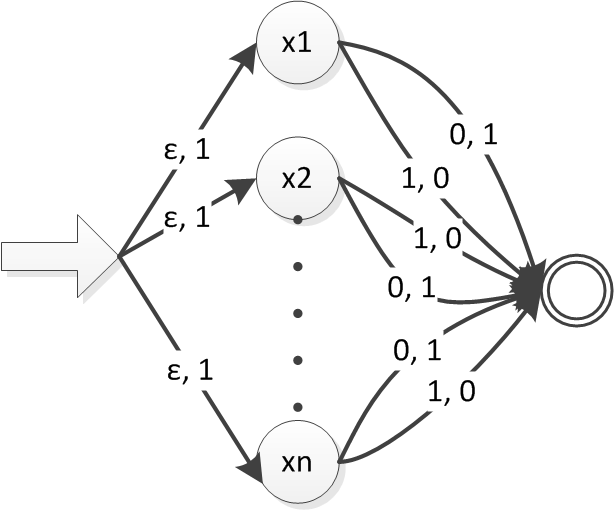
\includegraphics{n-and.png}
	\caption{Ultrametric query algorithm for n-ary AND.}
	  \label{n_and}
\end{figure}

The threshold value applied to the $p$-norm of the end state is 0: the answer 1 is given if the norm equals 0 and the answer 0 is returned if the norm is $>0$. The amplitude of the end state is 0 if and only if all of the arguments are 1. Note that this schema is valid for any prime number $>n$. 

The query complexity of an ultrametric algorithm can be further decreased if rational number tuples are allowed as amplitudes. Here the threshold is applied to the sum of p-norms of all of the components of the end state's amplitude (which again will be called the end state's amplitude's $p$-norm for simplicity). The class of such modified ultrametric query algorithms is called $n$-extended $p$-ultrametric query algorithms and were introduced by K. J\= eri\c n\v s \cite{Jer12}.

If an algorithm uses amplitude tuples, the graphical notation changes slightly. Now the second label on transitions is the transition's amplitude tuple, rather than just one amplitude.

An example to calculate function $f(x_1,x_2,x_3,x_4)=(x_1\vee x_2)\wedge (x_3\vee x_4)$ is shown in Fig. 2:

\begin{figure}
	\centering
	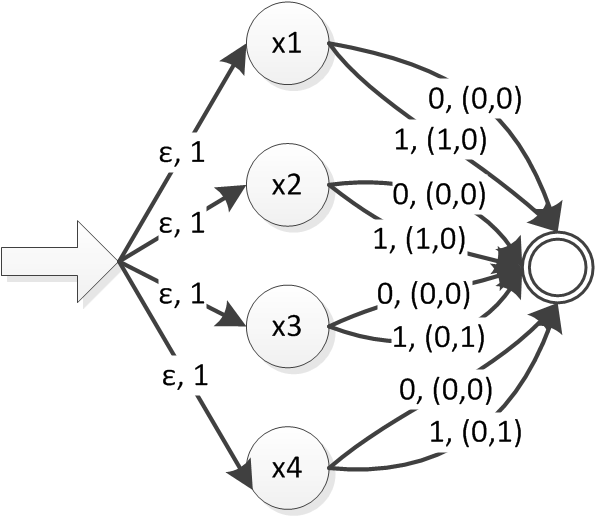
\includegraphics{or_and_or.png}
	\caption{Ultrametric algorithm for function $f(x_1,x_2,x_3,x_4 )=(x_1\vee x_2 )\wedge (x_3\vee x_4 )$}
	  \label{or_and_or}
\end{figure}

The threshold in this case is 2: the algorithm returns 1 if the end $p$-norm is $\geq2$.

\subsubsection{Permutations}
One class of permutations that are somewhat interesting with regard to their ultrametric realizations is permutations on finite geometries. If two ultrametric query algorithms for computing a function that tells whether a given permutation preserves a hypercube are compared from which one is an $n$-extended variation then it can be noted that while the $n$-extended variant has a smaller complexity it comes with a price of an enormous increase in the number of components of the amplitudes.

\begin{figure}
	\centering
	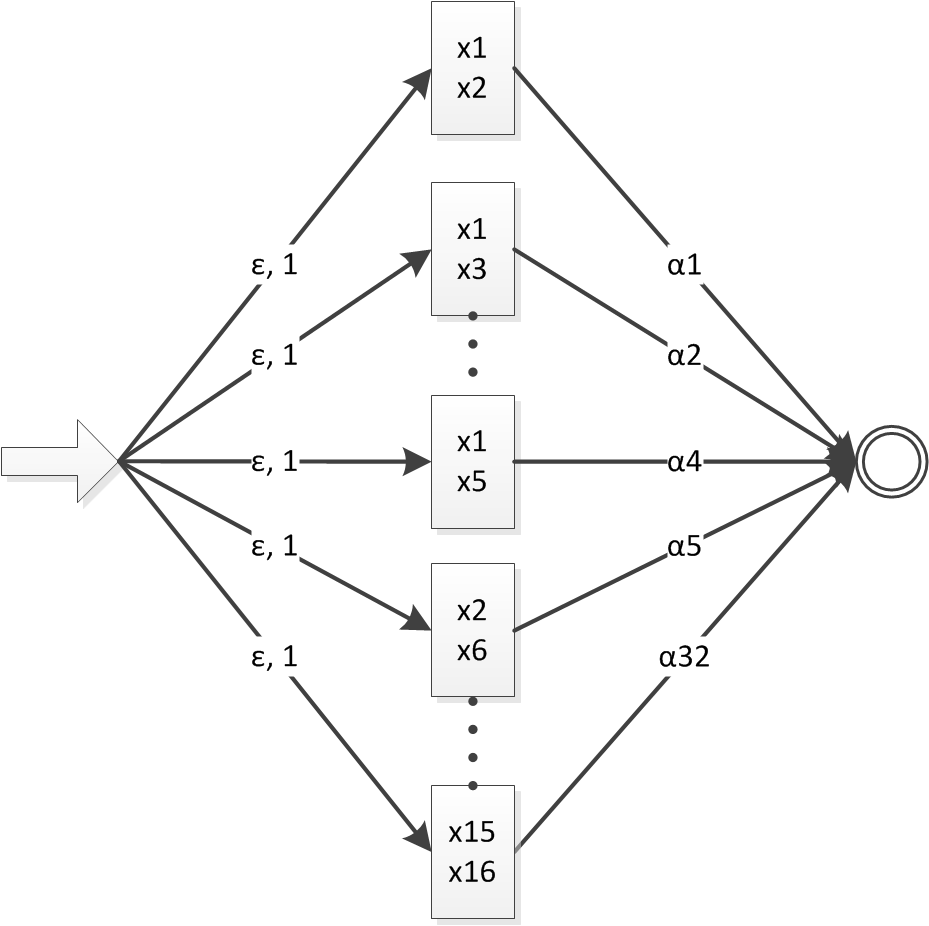
\includegraphics{hypercube_2block.png}
	\caption{Ultrametric query algorithm to compute whether a permutation preserves a hypercube with complexity of 2}
	  \label{hyper2}
\end{figure}

In Fig. 3 an ultrametric query algorithm that checks whether a given permutation preserves all of the edges of a hypercube is shown. The value $a_i$ is equal to 0 if the vertices corresponding to the $i$-th query block are connected and 1 otherwise. Here the threshold value can be picked as 0, since hypercube is preserved if and only if all of its edges are preserved. The schema works for any prime number $\geq 37$.

\begin{figure}
	\centering
	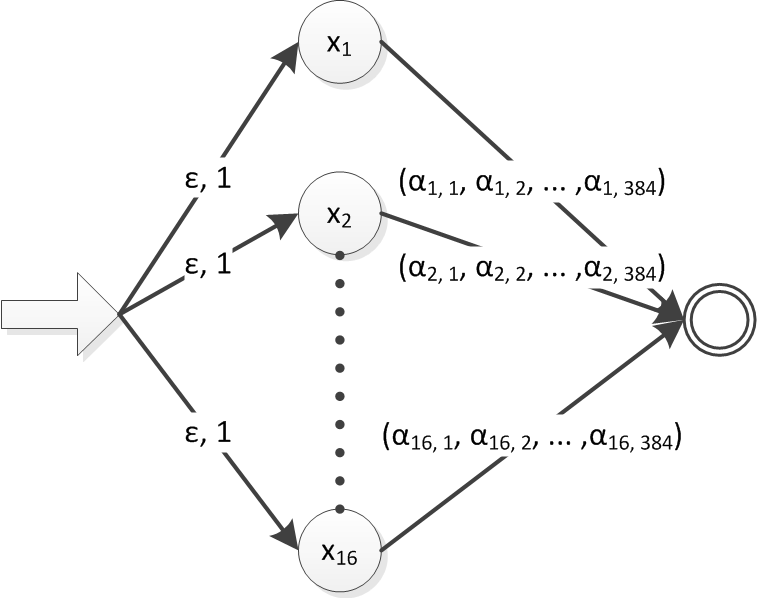
\includegraphics{hypercube_1block.png}
	\caption{$n$-extended ultrametric query algorithm to compute whether a permutation preserves a hypercube with complexity of 1}
	  \label{hyper1}
\end{figure}

In Fig. 4 a different approach is used. Here the given permutation is compared to a list of all valid permutations which are numbered from 1 to $n$. The values of amplitudes returned are
$$a_{i,j}=\begin{cases}
0, & \text{if in $j$-th permutation the value of $i$-th point is $x_i$} \\
1, & \text{otherwise}
\end{cases}$$
At the end the end state has amplitude $(\beta_1,\beta_2,\dots,\beta_n)$ where some number $\beta_i$ is equal to 0 if and only if the given permutation coincides with one of valid permutations. Since such $\beta_i$ can be only one the threshold can be chosen as 384 i.e. the number of valid permutations. The schema works for any prime number $\geq 17$.

As seen in the examples above, the decrease in complexity has been achieved at a cost of returning amplitudes of a very large length.

Now we will look at functions on permutations on graphs. If graph $G$ has vertices $1,2,3,\dots,k$ we say that a $k$-permutation preserves graph $G$ if for every pair $(i,j)$ the following holds - vertices $i$ and $j$ are connected with an edge in graph $G$ if and only if vertices $y_i$ and $y_j$ are connected in $G$.

\begin{theorem}
For every finite graph $G$ for every sufficiently large prime $p$ there exists a $p$-ultrametric query algorithm with complexity of 2 that checks whether the given permutation (contained in a black box) preserves graph $G$.
\end{theorem}
\begin{proof}
Since the graph $G$ is known we ask for every pair $(i,j)$ whether $(i,j)\in G$ iff $(y_i, y_j)\in G$. If so then we add $\frac{p}{r}$ to a designated state, where $r=\frac{k(k-1)}{2}$. If the permutation preserves G then the sum of amplitudes in the designated state equals $1$. Otherwise the sum is $<1$.
\qed
\end{proof}

\begin{theorem}
For every natural number $k$ there is such a graph $G_k$ with $k$ nodes that a deterministic query algorithm needs to make at least $(k-2)$ queries to determine whether a permutation preserves the graph.
\end{theorem}
\begin{proof}
The graph $G_k$ is a cycle of length $k$. If the permutation is not a cyclical shift $y_i = i+m(mod$ $k)$, it does not preserve the graph. If the permutation does preserve the graph but the values of two nodes are not yet known, there is still the possibility that the two values have been switched from the positions they would need to be for the permutation to preserve the graph, but if it is so, the permutation is not correct.
\qed
\end{proof}

\subsubsection{Other functions}
While the algorithms described earlier show a considerable decrease in complexity compared to deterministic query algorithms. An interesting result is existence of a class of functions for which the decrease in complexity can be achieved only for a specific prime number.

Let us consider a function
$$
f(x_n,x_{n-1},\dots,x_0)=\begin{cases}
1, & \text{if the number } \overline{x_nx_{n-1}\dots x_0} \text{ is divisible by 7} \\
0, & \text{otherwise}
\end{cases}
$$
where $(x_n,x_{n-1},\dots,x_0) \in \{0-9\}^{n+1}$.
\begin{figure}
	\centering
	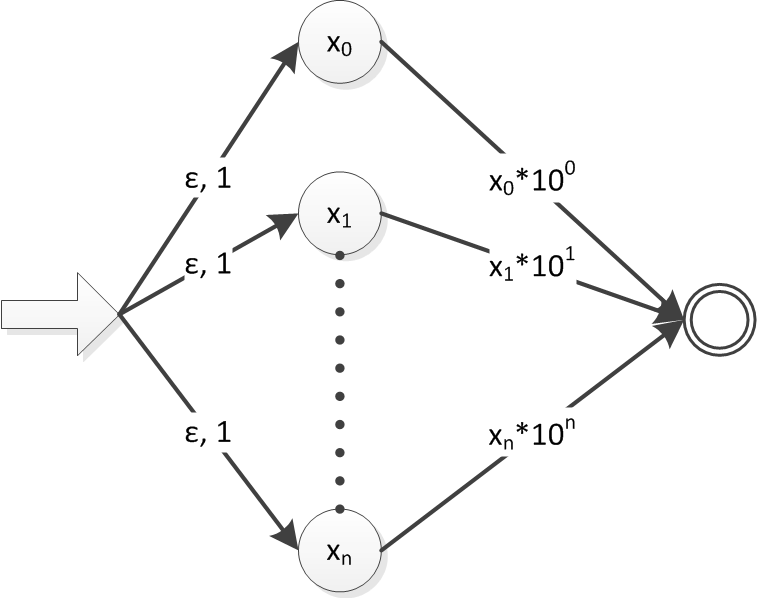
\includegraphics{divisibility.png}
	\caption{$7$-ultrametric query algorithm that checks number's divisibility by 7}
	  \label{div}
\end{figure}

In Fig. 5 it can be seen that the amplitude of the end state when the algorithm has finished is $a=x_n*10^n+x_{n-1}*10^{n-1}+\cdots+x_0*10^0$ i.e. the given number. By the definition of p-norm the value $||a||_7$ is $<1$ if $a$ a is divisible by 7 and exactly 1 if it is not, hence the threshold value can be chosen as 1.

Note that a similar $p$-ultrametric algorithm that checks whether a number is divisible by $p$ can be constructed for any prime number $p$.
%\bibliographystyle{te}

\bibliographystyle{unsrt}

\bibliography{bibliography.bib}

\end{document}


